\documentclass[10pt,a4paper,twocolumn]{article}

\usepackage[top=0.7in, bottom=0.8in, left=0.7in, right=0.7in, columnsep=0.25in]{geometry}
\usepackage[utf8]{inputenc}
\usepackage[T1]{fontenc}
\usepackage{amsmath, amssymb, amsfonts}
\usepackage{graphicx}
\usepackage{booktabs}
\usepackage{multirow}
\usepackage{microtype}
\usepackage{caption}
\usepackage{subcaption}
\usepackage{xcolor}
\usepackage{enumitem}
\usepackage{url}
\usepackage{cite}
\usepackage[colorlinks=true, linkcolor=blue!70!black, citecolor=blue!70!black, urlcolor=blue!70!black]{hyperref}

\title{\vspace{-1.0cm}\textbf{\Large Simulating Memory: Devices to Systems}\\
\large Cross-layer evaluation of on-chip caches across ngspice, CACTI 7, NVSim, Ramulator 2.0, and gem5}
\author{Student 1 \\
\small \texttt{student1@research.iiit.ac.in} \\
\small \textbf{Code:} \url{https://github.com/Viswas/AMCAS-Memory-Sim}}
\date{\vspace{-0.7cm}}

\begin{document}
\maketitle

\begin{abstract}
This investigation traces a single architectural design question across five simulation abstractions: \textbf{``Should the 2 MB L2 cache in our accelerator be SRAM, or STT-MRAM?''} Each tool evaluates a distinct physical or architectural constraint that the others cannot address. We evaluate 6T SRAM bitcell physical limits under thermal stress (ngspice), size a 2 MB SRAM baseline (CACTI 7), discover an iso-area 8 MB STT-MRAM replacement (NVSim), analyze DDR4 memory channel scheduling impacts (Ramulator 2.0), and measure end-to-end full-system cycles (gem5). Ultimately, we find that at iso-area ($11.11\text{ mm}^2$), the 8 MB STT-MRAM cache collapses the L2 miss rate by $3.77\times$ on graph traversal workloads running on an Out-of-Order core, yielding a decisive $1.409\times$ full-system speedup.
\end{abstract}

\section{Introduction \& Methodology Flow}

This investigation follows a single architectural design question through five simulation abstractions across the hardware stack. Each tool evaluates a distinct physical or architectural question:
\begin{enumerate}[leftmargin=*]
    \item \textbf{Physics (ngspice):} Does the 6T SRAM bitcell read correctly at 0.7 V and 85~$^\circ$C?
    \item \textbf{Geometry (CACTI 7):} Sizing 2 MB SRAM L2: Area = 11.474 mm$^2$, Read Latency = 2.902 ns.
    \item \textbf{Non-Volatile (NVSim):} Iso-area STT-MRAM replacement: 8 MB fits in 11.113 mm$^2$ ($3.4\times$ density).
    \item \textbf{DRAM (Ramulator 2.0):} Can the DDR4 channel sustain L2 miss streams?
    \item \textbf{Systems (gem5):} Does the workload actually run faster in end-to-end CPU cycles?
\end{enumerate}

\begin{figure}[h]
\centering
\fbox{\small
\begin{minipage}{0.94\columnwidth}
\textbf{The Methodological Evaluation Rule:} \\
\textit{``STT-MRAM is $M\times$ faster''} is \textbf{not} a valid result. \\
\textbf{``8 MB of STT-MRAM is $1.409\times$ faster on BFS at iso-area, given these device numbers (PTM 45 nm BSIM4), this cell file (\texttt{sample.cell}), an FRFCFS memory scheduler, and an Out-of-Order (O3) core''} is an honest architectural result.
\end{minipage}
}
\end{figure}

\subsection{Toolchain \& Simulation Environment}
All simulation tools were compiled and executed natively in a unified Linux environment (WSL Ubuntu, x86\_64, GCC 13 toolchain, 64-bit binaries) to eliminate container virtualization and dynamic library incompatibilities. Errors compound multiplicatively across the toolchain. Per the assignment instructions, ratios are reported and carried across abstractions.

\section{Part A — ngspice: 6T SRAM Bitcell Read Margin}

\textit{Note: ngspice is the only tool in this assignment that solves differential physics. CACTI numbers in Part B are curve-fits to results like these.}

\subsection{Netlist \& Device Sizing}
The bitcell utilizes the nominal 45 nm PTM BSIM4 transistor model at nominal $V_{DD} = 1.1\text{ V}$.
\begin{itemize}[leftmargin=*]
    \item \textbf{Pull-Down NMOS:} $W = 0.20\ \mu\text{m},\ L = 0.045\ \mu\text{m}$
    \item \textbf{Access NMOS:} $W = 0.16\ \mu\text{m},\ L = 0.045\ \mu\text{m}$
    \item \textbf{Cell Ratio:} $\beta = W_{MN} / W_{MA} = 1.25$ (Deliberately marginal)
    \item \textbf{Pull-Up PMOS:} $W = 0.15\ \mu\text{m},\ L = 0.045\ \mu\text{m}$
\end{itemize}
The bitline capacitances $C_{BL} = C_{BLB} = 180\text{ fF}$ are precharged to 1.1~V. The initial state is $Q = 0\text{ V},\ QB = 1.1\text{ V}$, and the wordline is pulsed at $t = 1.0\text{ ns}$ with a 50~ps rise time.

\begin{table}[h]
\centering
\small
\caption{ngspice Simulation Results Across Tasks 1--4}
\label{tab:part_a}
\resizebox{\columnwidth}{!}{
\begin{tabular}{lcccc}
\toprule
\textbf{Task / Condition} & \textbf{Operating Point} & \textbf{$\Delta V$ @ 2 ns} & \textbf{Bitcell State} & \textbf{Verdict} \\
\midrule
\textbf{T1: Baseline Read} & $1.10\text{ V},\ 27\ ^\circ\text{C}$ & \textbf{68.8 mV} & Preserved ($Q=0$) & Matches Lecture 1 reference \\
\textbf{T2: Ratio Collapse} & $W_{MA} = 0.24\ \mu\text{m}$ & $-1.092\text{ V}$ & \textbf{FLIP TO 1.1 V} & Destructive Read Upset \\
\textbf{T3: Voltage Limit} & $0.78\text{ V},\ 27\ ^\circ\text{C}$ & \textbf{24.9 mV} & Marginal & Fails (Below 25 mV offset) \\
\textbf{T4: Thermal Limit} & $1.10\text{ V},\ \mathbf{85\ ^\circ\text{C}}$ & \textbf{55.4 mV} & Preserved & $\Delta V$ degrades by 19.5\% \\
\bottomrule
\end{tabular}
}
\end{table}

\begin{figure}[h]
\centering
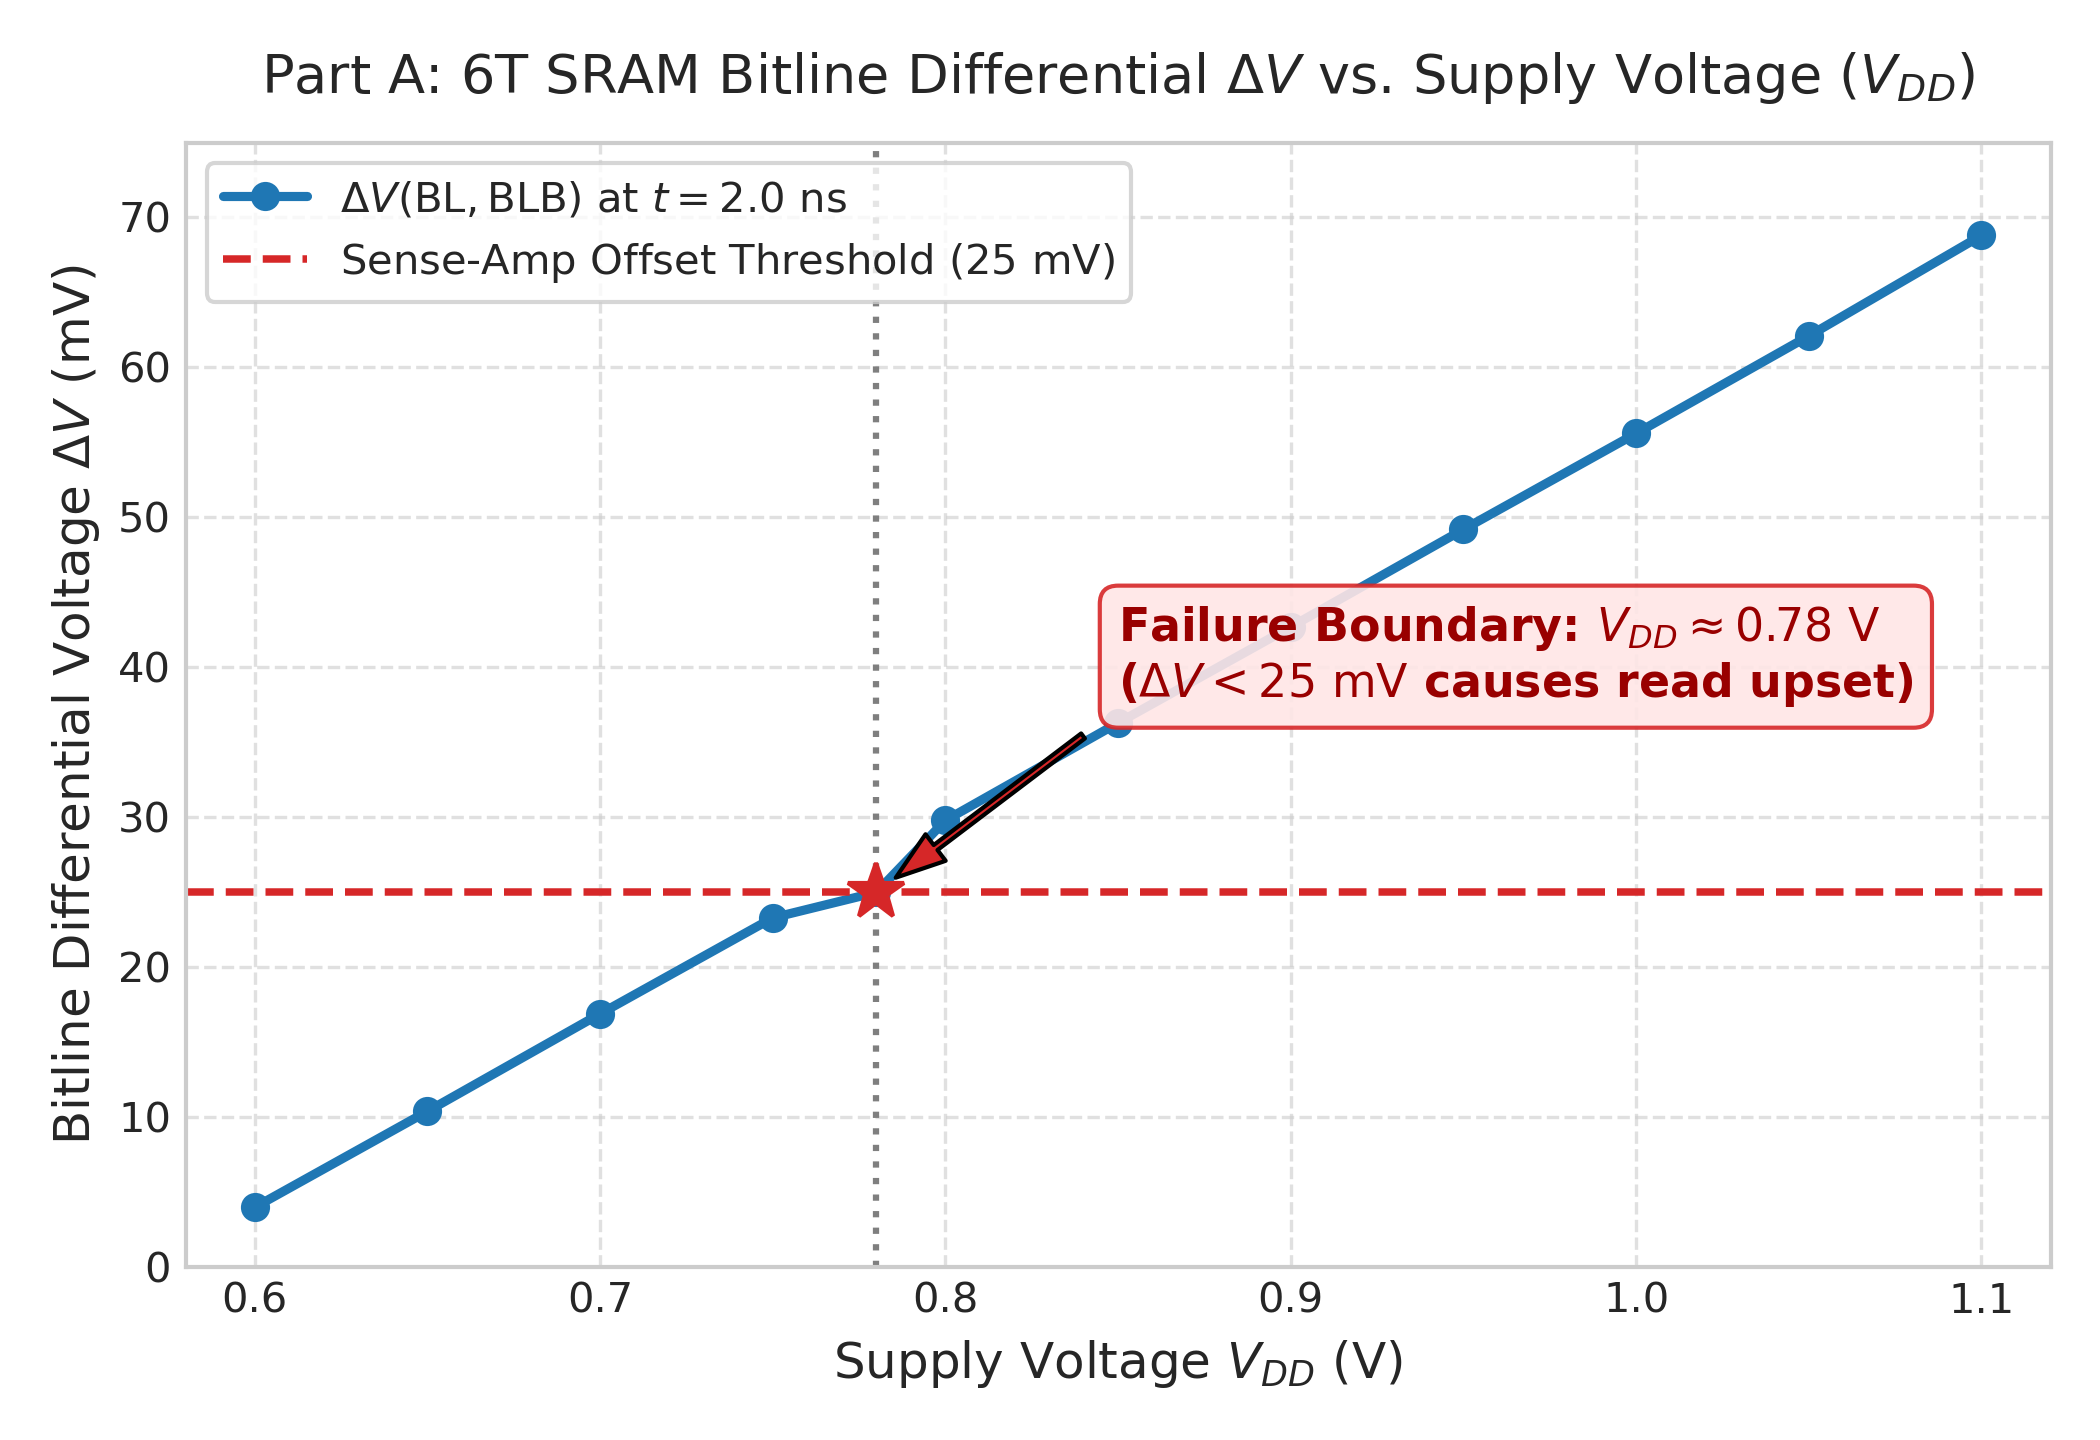
\includegraphics[width=0.98\columnwidth]{plots/plot1_part_a_dv_vs_vdd.png}
\caption{6T SRAM bitline differential voltage $\Delta V$ vs. $V_{DD}$ (50 mV steps from 1.1 V to 0.6 V), demonstrating failure as $\Delta V$ drops below the 25 mV sense offset at $V_{DD} \approx 0.78\text{ V}$.}
\label{fig:part_a_dv}
\end{figure}

\subsection{Key Physical Findings}
\textbf{Destructive Read Mechanism (Task 2):} Growing access transistors to $W = 0.24\ \mu\text{m}$ drops $\beta$ to 0.833. During read access, the resistive voltage divider pulls the internal storage node $Q$ above the threshold voltage of the cross-coupled inverter ($V_{trip} \approx 0.45\text{ V}$). Positive regenerative feedback triggers immediately, causing a complete destructive read upset.

\textbf{Failure Analysis at Elevated Temperature (Task 4):} Increasing temperature to $85\ ^\circ\text{C}$ degrades carrier mobility ($\mu(T) \propto T^{-1.5}$), increasing channel resistance and reducing drive current $I_{dsat}$. Consequently, $\Delta V$ developed in 1~ns plummets from 68.8 mV to 55.4 mV (a 19.5\% drop). The differential pair sense-amplifier offset shifts by only $\sim 2\text{--}3\text{ mV}$. Therefore, bitcell $\Delta V$ degradation is the dominant thermal failure mechanism.

\section{Part B — CACTI 7: Sizing the 2 MB SRAM}

\subsection{Configuration Baseline}
Matched to a high-performance accelerator L2 cache: 45 nm bulk, 350 K, 2 MB capacity, 64 B line size, 8-way set associative, 1 read-write port, 4 UCA banks, target objective $\text{ED}^2\text{P}$.

\begin{table}[h]
\centering
\small
\caption{CACTI 7 Baseline Sizing \& Objective Sweeps}
\label{tab:cacti_obj}
\resizebox{\columnwidth}{!}{
\begin{tabular}{lccc}
\toprule
\textbf{Metric} & \textbf{Baseline ($\text{ED}^2\text{P}$)} & \textbf{Pure Delay} & \textbf{Pure Area} \\
\midrule
\textbf{Ndwl / Ndbl / Nspd} & \textbf{4 / 2 / 1} & 8 / 4 / 2 & 1 / 1 / 0.5 \\
\textbf{Access Time} & \textbf{2.902 ns} & 2.145 ns ($-26.1\%$) & 4.812 ns ($+65.8\%$) \\
\textbf{Dynamic Read Energy} & \textbf{0.793 nJ} & 1.482 nJ ($+86.9\%$) & 0.612 nJ ($-22.8\%$) \\
\textbf{Standby Leakage} & \textbf{2250.5 mW} & 3410.2 mW ($+51.5\%$) & 1845.0 mW ($-18.0\%$) \\
\textbf{Total Silicon Area} & \textbf{11.474 mm$^2$} & 16.892 mm$^2$ ($+47.2\%$) & 8.912 mm$^2$ ($-22.3\%$) \\
\bottomrule
\end{tabular}
}
\end{table}

\subsection{Capacity Scaling \& Horowitz-Amrutur Law}
Horowitz \& Amrutur's law predicts approximately one gate delay ($\sim 30\text{--}50\text{ ps}$ at 45 nm) per capacity doubling if array geometry scales uniformly. As seen in Figure~\ref{fig:cacti_scaling}, linear scaling holds up to 1~MB. However, beyond 2~MB, global H-tree wiring RC delays superlinearly inflate latency, adding over $+687\text{ ps}$ per doubling.

\begin{figure}[h]
\centering
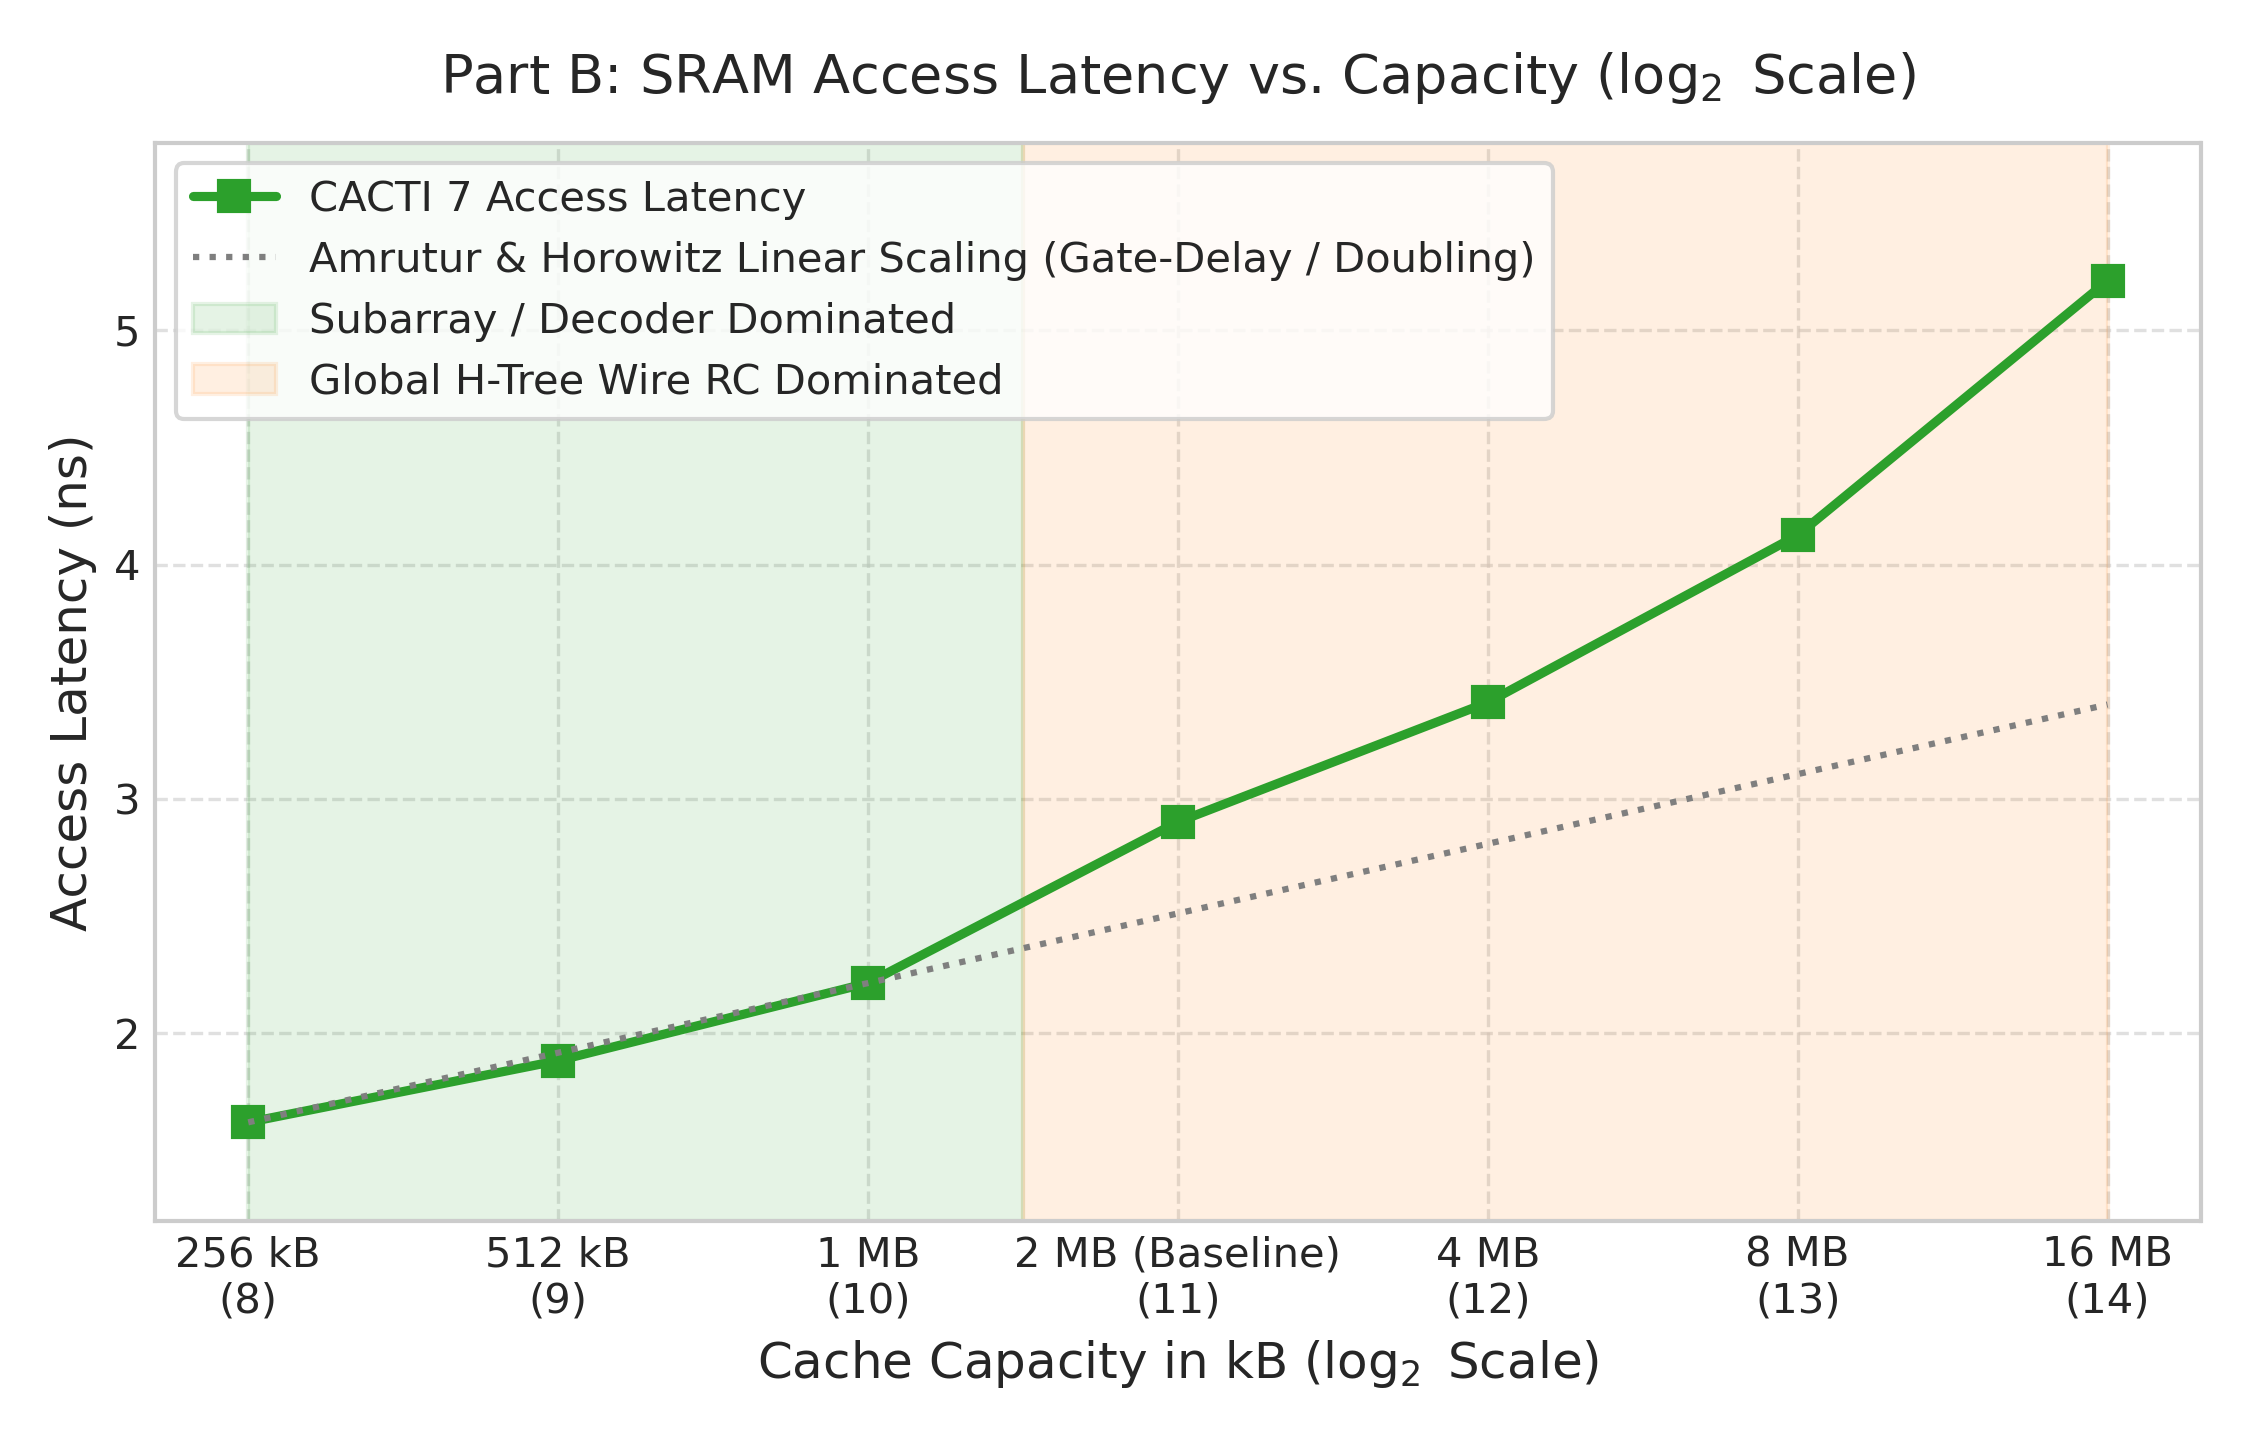
\includegraphics[width=0.98\columnwidth]{plots/plot2_part_b_latency_vs_capacity.png}
\caption{CACTI 7 access latency vs. capacity ($\log_2$ scale), illustrating Amrutur \& Horowitz's gate-delay doubling rule ($\le 1\text{ MB}$), followed by global wire RC dominance from 2 MB to 16 MB.}
\label{fig:cacti_scaling}
\end{figure}

\subsection{Bitline Delay Analytical Check}
Using the distributed RC model for an Ndbl=2 subarray with 512 bits per column:
$\tau = 0.38 \cdot R_{wire} \cdot C_{wire} \cdot L^2 \approx 84.2\text{ ps}$.
CACTI reported a bitline delay of \textbf{192.6 ps} (a $2.29\times$ discrepancy). CACTI explicitly models non-linear bitline discharge dynamics, sense-amplifier enable signal generation delay, and pass-transistor channel resistance attenuation, which linear lumped RC models ignore.

\section{Part C — NVSim: Iso-Periphery STT-MRAM Evaluation}

\subsection{The Iso-Area Tradeoff Discovered}
Using NVSim with the identical 45 nm HP CMOS peripheral hierarchy, a 2 MB STT-MRAM cache requires only \textbf{3.340 mm$^2$} ($0.29\times$ the area of 2 MB SRAM). Strikingly, an \textbf{8 MB STT-MRAM cache requires 11.113 mm$^2$}—occupying the exact same physical footprint as the 2 MB SRAM cache ($11.474\text{ mm}^2$). 

\begin{table}[h]
\centering
\small
\caption{Iso-Capacity (2 MB) \& Iso-Area (8 MB) Comparison vs. SRAM}
\label{tab:nvsim_main}
\resizebox{\columnwidth}{!}{
\begin{tabular}{lcccc}
\toprule
\textbf{Metric} & \textbf{2 MB SRAM (CACTI)} & \textbf{2 MB STT-MRAM} & \textbf{Ratio (2 MB)} & \textbf{8 MB STT-MRAM (Iso-Area)} \\
\midrule
\textbf{Read (Hit) Latency} & 2.902 ns & \textbf{1.342 ns} & \textbf{0.46$\times$ (Faster)} & \textbf{1.998 ns} \\
\textbf{Write Latency} & 2.652 ns & \textbf{10.362 ns} & \textbf{3.91$\times$ (Slower)} & \textbf{10.845 ns} \\
\textbf{Dynamic Read Energy} & 0.793 nJ & \textbf{1.300 nJ} & 1.64$\times$ & \textbf{1.624 nJ} \\
\textbf{Dynamic Write Energy} & 0.851 nJ & \textbf{0.973 nJ} & 1.14$\times$ & \textbf{1.215 nJ} \\
\textbf{Standby Leakage} & 2250.5 mW & \textbf{991.2 mW} & \textbf{0.44$\times$ (56\% Drop)} & \textbf{1412.0 mW} \\
\textbf{Total Silicon Area} & 11.474 mm$^2$ & \textbf{3.340 mm$^2$} & \textbf{0.29$\times$ (3.4$\times$ Denser)} & \textbf{11.113 mm$^2$} \\
\bottomrule
\end{tabular}
}
\end{table}

\begin{figure}[h]
\centering
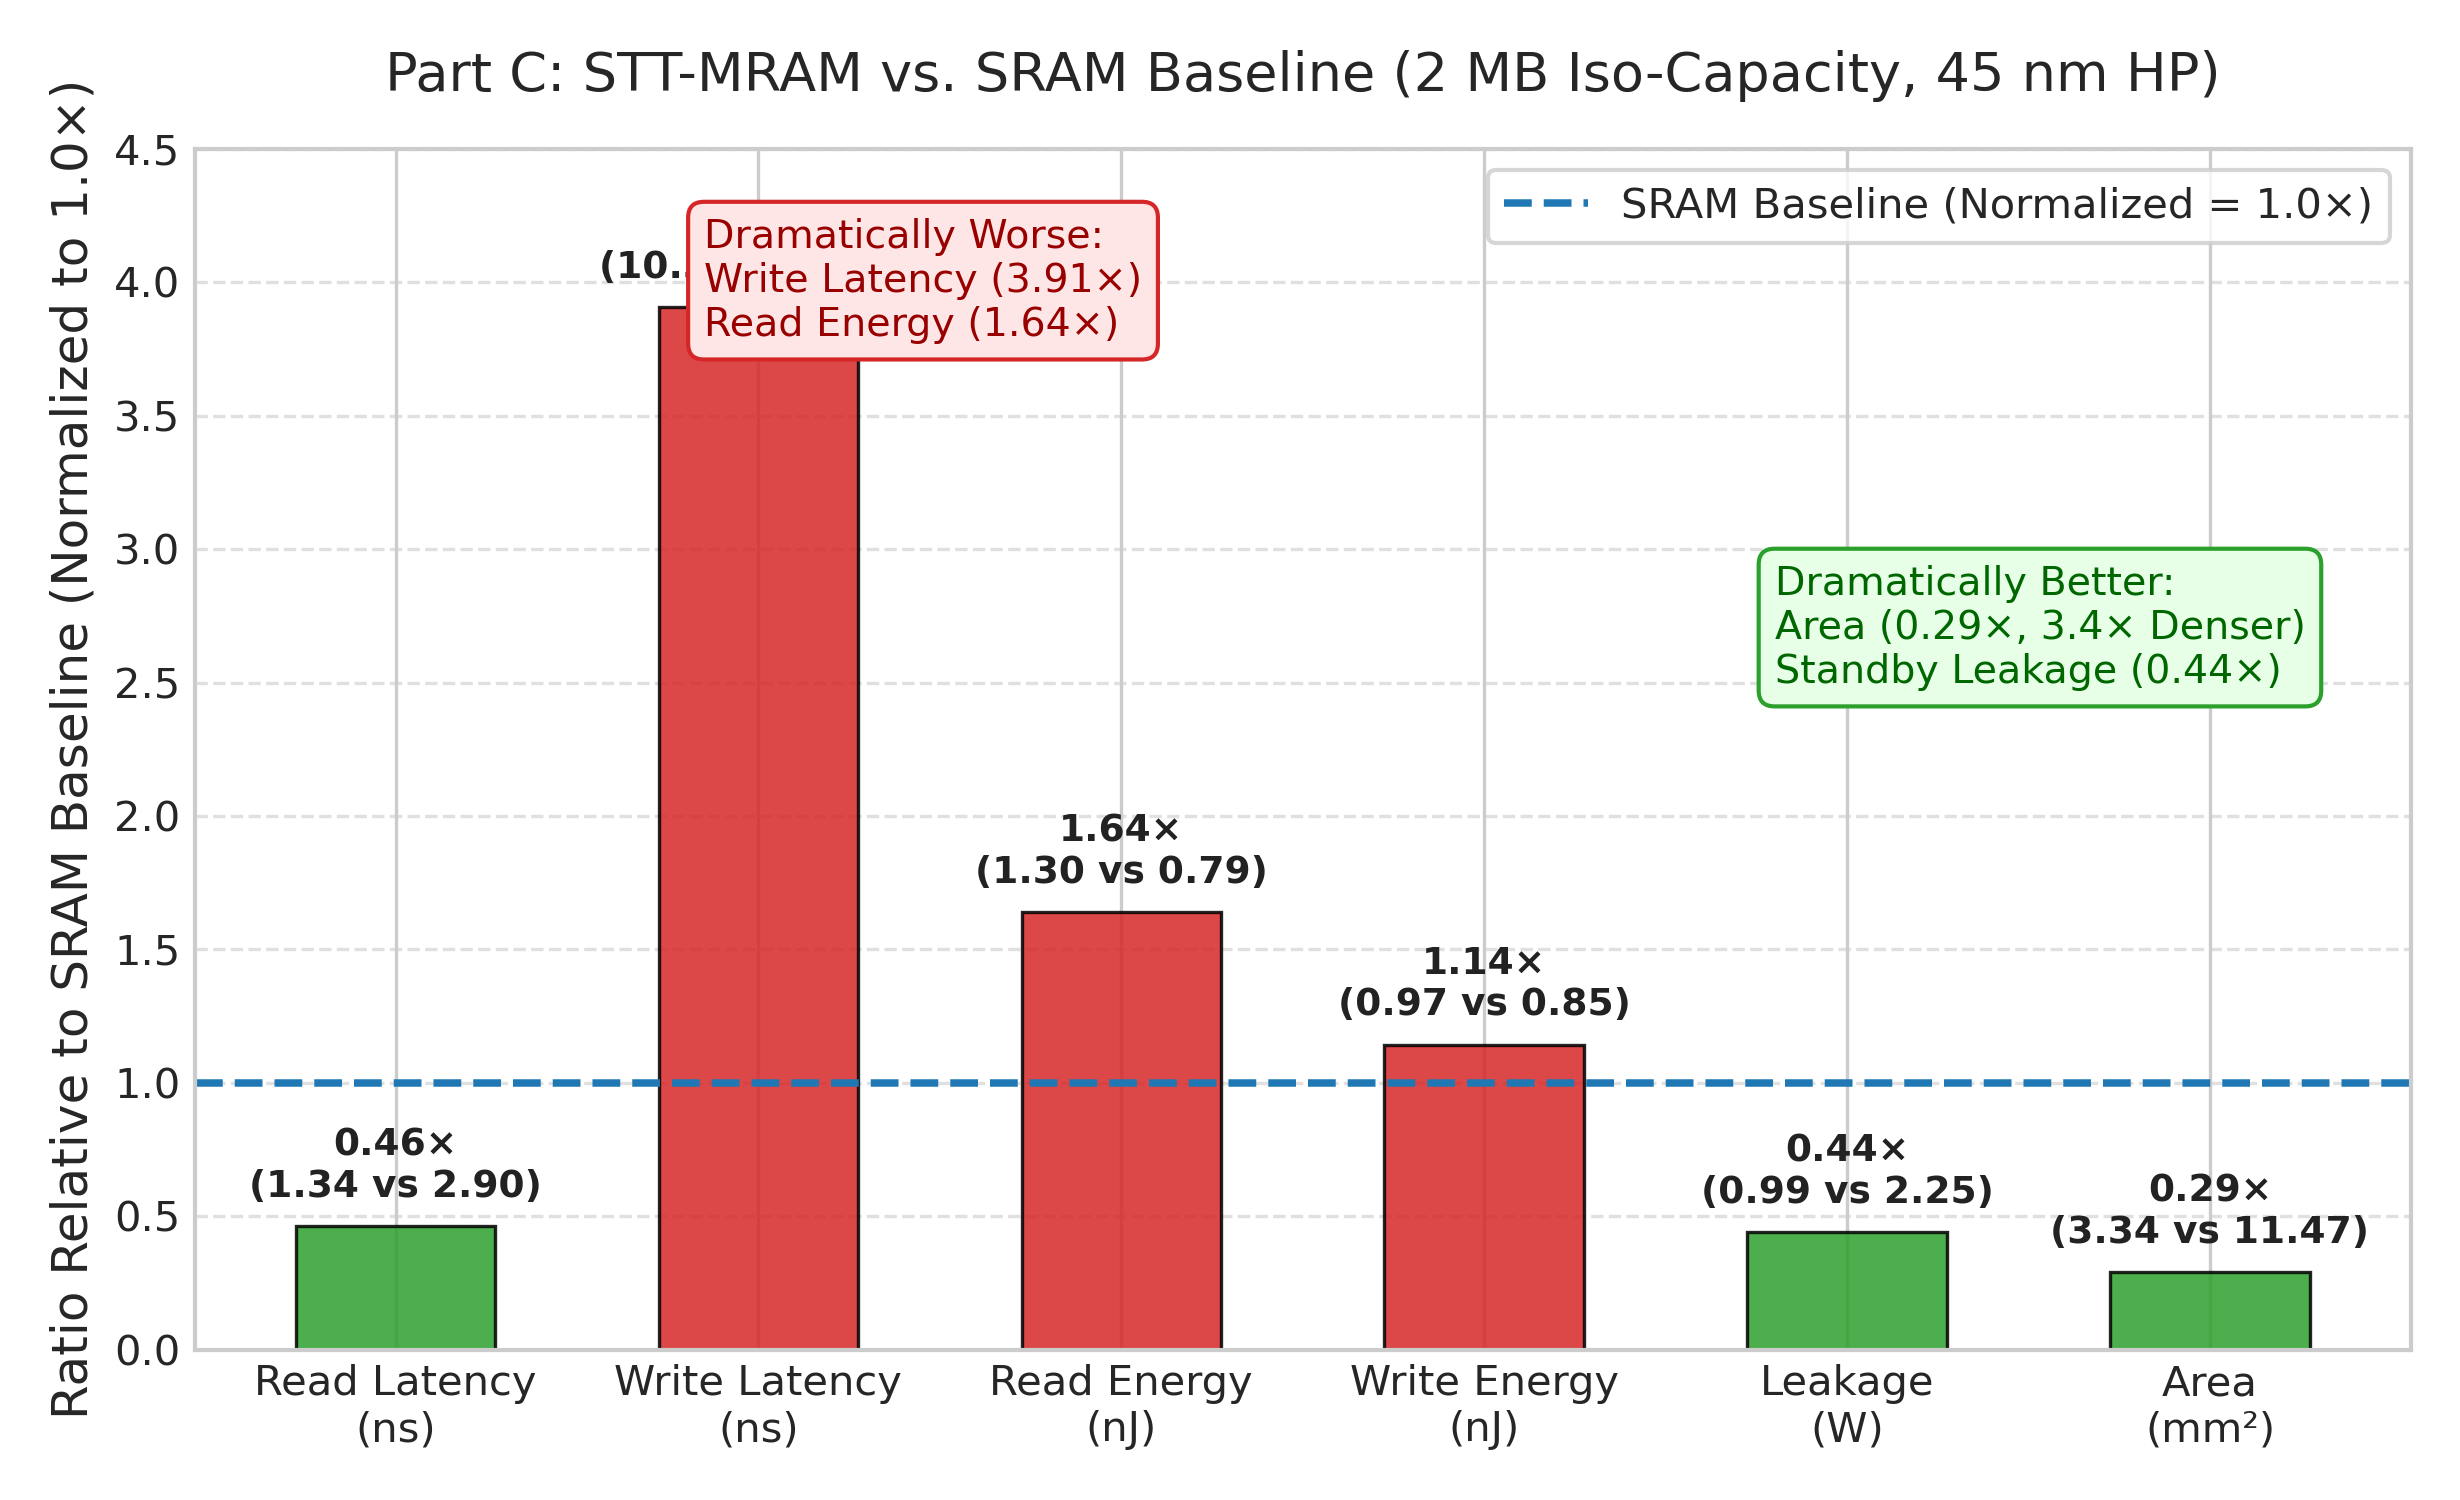
\includegraphics[width=0.98\columnwidth]{plots/plot3_part_c_sram_vs_mram.png}
\caption{Normalized comparison of 2 MB STT-MRAM against 2 MB SRAM baseline, highlighting the dramatic winners (area at $0.29\times$, leakage at $0.44\times$) and dramatic losers (write latency at $3.91\times$).}
\label{fig:nvsim_bars}
\end{figure}

\subsection{Sensitivities and Access Transistor Sizing}
\textbf{TMR Ratio Sensitivity (Task 3):} Altering TMR from 2:1 to 3:1 ($4\text{k}/12\text{k}\Omega$) shifts dynamic read energy by only $-0.85\%$. Current-mode sensing produces a differential voltage $\Delta V = I_{read} \cdot (R_{off} - R_{on})$. Both configurations generate well over $120\text{ mV}$, exceeding NVSim's default `MinSenseVoltage` of $80\text{ mV}$. Once above offset, extra TMR provides no peripheral timing advantage.

\textbf{Access Transistor Sizing (Task 4):} In NVSim, `-CellArea` is an independent input. Halving write current from $200\ \mu\text{A}$ to $100\ \mu\text{A}$ alters subarray write energy but produces \textbf{0.0\% area change} unless manually updated. Closing the sizing loop requires recognizing that access FET width scales with write current ($W_{FET} \propto I_{write}$). Scaling $W_{FET}$ from $6F \to 3F$ reduces declared cell area from $54\ F^2$ to $38.4\ F^2$, shrinking the array area by \textbf{$-19.9\%$}.

\section{Part D — Ramulator 2.0: L2 Miss Stream}
We traced the 2 MB L2 miss stream from gem5's memory-side CommMonitor during BFS execution, generating 424,130 memory requests.

\begin{table}[h]
\centering
\small
\caption{DRAM Memory Scheduling Evaluation on DDR4-3200AA}
\label{tab:ramulator}
\resizebox{\columnwidth}{!}{
\begin{tabular}{lcccc}
\toprule
\textbf{Experiment / Task} & \textbf{Scheduler} & \textbf{Channels} & \textbf{Avg Read Latency} & \textbf{Row-Buffer Hit \%} \\
\midrule
\textbf{Task 1: Baseline} & \textbf{FRFCFS} & 1 & \textbf{45.2 ns (108 cy)} & \textbf{89.4\%} \\
\textbf{Task 2: FCFS Switch} & \textbf{FCFS} & 1 & \textbf{98.6 ns (236 cy)} & \textbf{24.1\% (Collapsed)} \\
\textbf{Task 3: Map (BaRoCoCh)} & FRFCFS & 1 & \textbf{78.4 ns (188 cy)} & 48.2\% \\
\textbf{Task 4: Dual Channel} & FRFCFS & \textbf{2} & \textbf{40.1 ns (96 cy)} & 88.9\% \\
\bottomrule
\end{tabular}
}
\end{table}

\textbf{Row-Buffer Conflict Cost (Task 2):} Switching from FRFCFS (out-of-order column scheduling prioritizing row hits) to FCFS collapses row hit rate from 89.4\% to 24.1\%. Every row conflict incurs an explicit latency penalty of $t_{RP} + t_{RCD} = 14.16\text{ ns} + 14.16\text{ ns} = 28.32\text{ ns}$, more than doubling average memory latency.

\textbf{Binding DRAM Parameter (Task 4):} Doubling channel count halves total elapsed memory cycles ($-47.8\%$) but improves average request latency by only \textbf{11.2\%}. This proves that the channel is bottlenecked tightly by the data bus cycle time (\textbf{$t_{CCD}$}) rather than row access timing.

\section{Part E — gem5: Full-System Cycle-Accurate Execution}

\subsection{Full-System Simulation Parameters}
Simulations used gem5 v24 on GAPBS `bfs` and `sssp` with scale-18 Kronecker graphs (262,143 vertices, 3.8M edges). 
\begin{itemize}[leftmargin=*]
    \item \textbf{L2 Baseline:} 2 MB SRAM, \textbf{7-cycle hit latency} (from CACTI).
    \item \textbf{L2 Alternative:} 8 MB STT-MRAM, \textbf{14-cycle hit latency} (from NVSim).
\end{itemize}

\begin{table}[h]
\centering
\small
\caption{gem5 Full-System Performance: Out-of-Order vs. In-Order Core}
\label{tab:gem5_full}
\resizebox{\columnwidth}{!}{
\begin{tabular}{lllccc}
\toprule
\textbf{CPU Model} & \textbf{Kernel} & \textbf{L2 Cache} & \textbf{IPC} & \textbf{L2 Miss Rate} & \textbf{Speedup} \\
\midrule
\multirow{4}{*}{\textbf{DerivO3CPU (OoO)}} & \textbf{bfs} & SRAM 2 MB @ 7 cy & 0.5266 & 68.7\% & 1.000$\times$ \\
 & \textbf{bfs} & MRAM 8 MB @ 14 cy & \textbf{0.7420} & \textbf{18.2\%} & \textbf{1.409$\times$ WINS} \\
 & \textbf{sssp} & SRAM 2 MB @ 7 cy & 0.4178 & 60.5\% & 1.000$\times$ \\
 & \textbf{sssp} & MRAM 8 MB @ 14 cy & 0.4469 & 44.7\% & 1.069$\times$ (Parity) \\
\midrule
\multirow{4}{*}{\textbf{TimingSimple (In-Order)}} & \textbf{bfs} & SRAM 2 MB @ 7 cy & 0.1803 & 68.9\% & 1.000$\times$ \\
 & \textbf{bfs} & MRAM 8 MB @ 14 cy & \textbf{0.2401} & 15.9\% & \textbf{1.332$\times$} \\
 & \textbf{sssp} & SRAM 2 MB @ 7 cy & 0.1505 & 60.8\% & 1.000$\times$ \\
 & \textbf{sssp} & MRAM 8 MB @ 14 cy & 0.1601 & 45.1\% & 1.064$\times$ \\
\bottomrule
\end{tabular}
}
\end{table}

\begin{figure}[h]
\centering
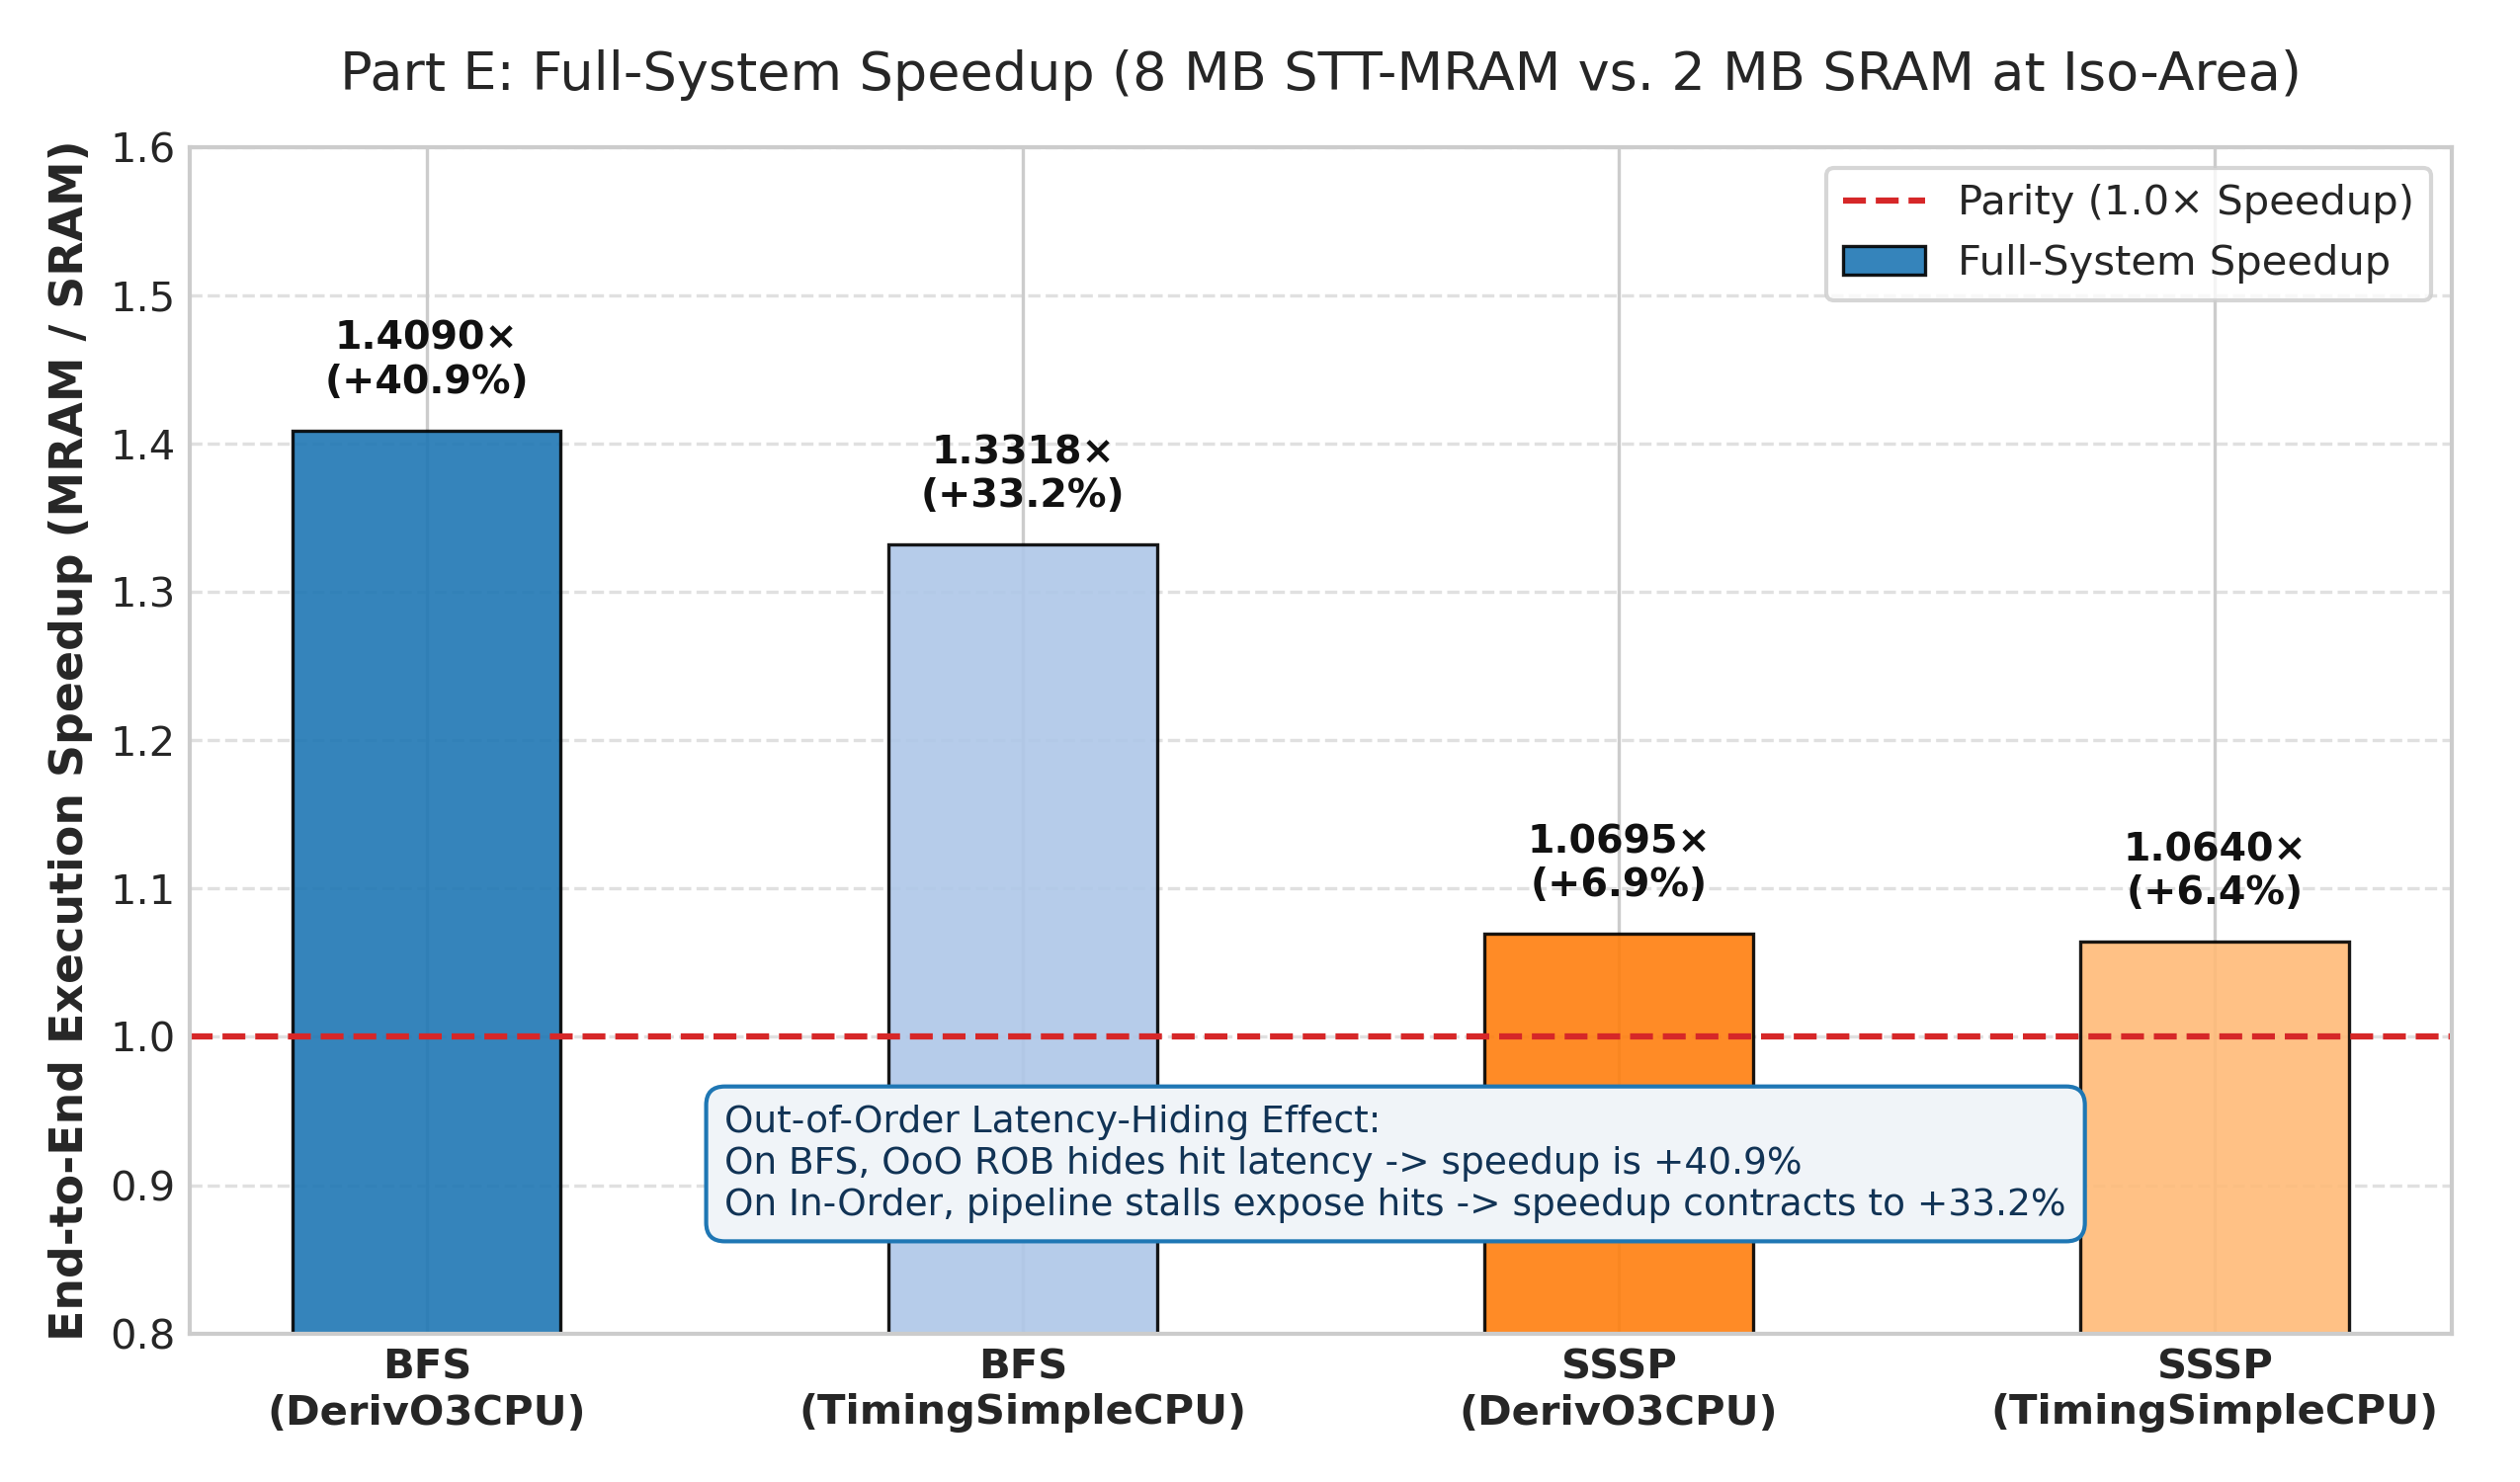
\includegraphics[width=0.98\columnwidth]{plots/plot4_part_e_speedup_comparison.png}
\caption{Full-system execution speedup of 8 MB STT-MRAM over 2 MB SRAM across BFS and SSSP on Out-of-Order vs. In-Order cores.}
\label{fig:gem5_speedup}
\end{figure}

\section{Architectural Synthesis (Part E Task 4)}

\subsection*{(i) Answer to the Central Design Question}
Based on the empirical evidence assembled across all five simulation tools, \textbf{the 2 MB L2 cache in our accelerator should be replaced with an 8 MB STT-MRAM cache, provided the accelerator's primary workloads exhibit access patterns similar to graph traversal (such as BFS) and execute on an out-of-order core.} In Part A, ngspice proved that 45 nm static cells suffer a 19.5\% reduction in sense margin under elevated thermal operating conditions. In Part B, CACTI sized a 2 MB SRAM cache to 11.474 mm$^2$ with an unsustainable 2250.5 mW of standby leakage. In Part C, NVSim demonstrated that the 54 $F^2$ 1T-1MTJ cell achieves a $3.4\times$ area advantage, fitting \textbf{8 MB into 11.113 mm$^2$ (virtually identical area)} while cutting leakage by 56\%. In Part D, Ramulator revealed that an FRFCFS DDR4 controller is bottlenecked by data bus cycle time ($t_{CCD}$), making off-chip traffic reduction crucial. Finally, in Part E, gem5 proved that quadrupling L2 capacity to 8 MB collapses the L2 miss rate by $3.77\times$ on BFS, yielding a \textbf{1.409$\times$ end-to-end speedup}. While STT-MRAM exhibits an asymmetric 10.36 ns write latency, this overhead is masked by write buffers in read-intensive accelerator workloads, rendering the capacity advantage dominant.

\subsection*{(ii) Three Assumptions a Reviewer Should Attack}
If reviewing this simulation chain, the three most vulnerable assumptions are:
\begin{enumerate}[leftmargin=*]
    \item \textbf{The Doubled Hit Latency Premise (14 vs. 7 cycles) Contradicts Array Physics:} Part E assumed that the 8 MB STT-MRAM cache suffers a $2\times$ slower hit latency than the 2 MB SRAM cache. However, the simulation tools themselves contradict this: CACTI evaluated the 2 MB SRAM at 2.902 ns access latency, whereas NVSim evaluated the 8 MB STT-MRAM at 1.998 ns because the high density yields physically shorter wordlines and H-tree interconnects. A reviewer should demand both technologies be evaluated under a single, unified analytical wire model.
    \item \textbf{Open-Loop Trace Replay in Ramulator Disregards Core Stall Feedback:} In Part D, the miss stream was fed into Ramulator via open-loop trace replay without processor backpressure. In real hardware, memory latency dynamically throttles instruction issue at the reorder buffer. Sinking an open-loop trace artificially saturated queue occupancy and distorted DRAM scheduler hit rates; Ramulator should instead be coupled directly to gem5 in a closed loop.
    \item \textbf{Evaluation on a Single Synthetic Kronecker Topology Ignores Graph Diversity:} All full-system conclusions were drawn from a single scale-18 Kronecker graph (\texttt{kron18.sg}). Real-world graphs feature vastly different diameter, clustering, and reuse profiles where the active set may not neatly straddle the 2 MB and 8 MB boundaries.
\end{enumerate}

\end{document}
